% !TeX spellcheck = en_GB
% !TEX root = ../thesis.tex


\chapter{Second-order topological modes in continuous media} \label{ch:hoti} 


\begin{chapterabstract}
	In Chapter \ref{ch:symmetry}, we introduced a framework to investigate band spectrum degeneracies using the methods of group theory.	
	In particular, we saw that a sixfold-symmetric lattice may be perturbed in a variety of ways, each of which produces a different gap-opening term at the $\boldsymbol{K}$ point of the Brillouin zone. In this Chapter, we show that combining the deformations in a single system emulates the 2D Jackiw-Rossi model of a topological vortex, where 0D in-gap bound modes are guaranteed to exist. Adapting the analytic approach from Chapter \ref{ch:symmetry} for numerical work, we show how to extract the signature topological properties from finite-element simulations. We then numerically demonstrate the existence of bound modes in a Jackiw-Rossi vortex. Our scheme enables the realization of second-order topology in a wide range of experimental systems and further optimization of the bound mode characteristics. 
	%
	\tcblower
	%
	The bulk of this chapter is adapted from Ref.~\cite{Kosata_2021}.
\end{chapterabstract}

We consider two distinct perturbations of a \textit{p6m}-symmetric structure, namely the breaking of inversion and translation symmetries, whose representation matrices we found in Sec.~\ref{sec:symm_groups}. These anticommute and thus correspond to fundamentally distinct gap-opening terms -- the building blocks of the Jackiw-Rossi model. For concreteness, we assume a dielectric implementation of the scheme; we stress however that our analysis holds for any patterned 2D linear medium. 

\section{The Jackiw-Rossi model} 
Second-order topological insulators are $d$-dimensional systems which may feature defect modes of dimension $d-2$. 
An instance thereof is found in the $d=2$ Jackiw-Rossi Hamiltonian of a topological vortex, which can be implemented by deforming the tight-binding model of graphene~\cite{Hou_2007}. Emulating this model has successfully demonstrated the creation of 0D modes at topological vortices in photonic~\cite{Gao_2019, Gao_2020,  Yang_2020} and elastic~\cite{Xiaoxiao_2021} devices. The 2D Jackiw-Rossi Hamiltonian reads
\begin{equation} \label{eq:hoti_H}
H = \boldsymbol{\gamma} \vdot \vb{k} + \boldsymbol{\Gamma} \vdot \boldsymbol{m}(\vb{r})\,,
\end{equation}
where $\vb{k} = (k_x, k_y)$ are quasimomenta, and $\boldsymbol{m}(\vb{r})=(m_1(\vb{r}),m_2(\vb{r}))$ are mass terms that can change in space $\vb{r}=(x,y)$. The four $4 \times 4$ matrices, $\boldsymbol{\gamma} = (\gamma_x, \gamma_y)$ and $\boldsymbol{\Gamma} = (\Gamma_1, \Gamma_2)$, anticommute with one another.
If either of the mass terms $m_1$ or $m_2$ is nonzero, the spectrum of $H$ is gapped around zero energy.

We first discuss the case where one mass term (e.g., $m_2$) vanishes and the other switches signs in space [e.g., $m_1 = \abs{m}\, \text{sgn}(x)$], thus defining a domain wall at $x=0$. The distinct band topology of the two bulk phases then defines a topological defect and a band inversion occurs across $x=0$. This gives us two copies of the Jackiw-Rebbi model~\cite{Jackiw_1976, Wu_Hu_2015}, introduced in Chapter \ref{ch:intro} and the system admits a $\mathbb{Z}_2$ invariant~\cite{Kane_2005b, Qi_2008}. Correspondingly, two counter-propagating 1D edge states appear at the domain wall. Depending on the eigenbasis of the gapping term, we thus obtain the states associated with either the quantum spin Hall effect (QSHE) or the quantum valley Hall effect (QVHE).

Allowing instead both masses to vary over a space-dependent closed path defines a defect centred at a point\footnote{For a more complete discussion of the defect dimensions and corresponding topological invariants, see Refs.~\cite{Kosata_2021, Teo_2010}.}. The Hamiltonian is then characterised by a $\mathbb{Z}$ topological invariant associated with the winding number $n$ of $\boldsymbol{m}(\vb{r})$. Defining $m_1 + i m_2 = \abs{\boldsymbol{m}} e^{i \theta}$, the winding number reads
\begin{equation} \label{eq:invariant}
n = \frac{1}{2\pi} \oint_{S^1} d\theta\,,
\end{equation}
where $S^1$ denotes the closed path. At such a topological vortex, $n$ zero-dimensional bound modes are found. Systems with $\abs{n} > 0$ can be constructed within the TB model of graphene, where $m_1$ and $m_2$ are generated by spatial perturbations of the six-site unit cell~\cite{Hou_2007}. We also emphasize that this model is topologically equivalent to the well-known Benalcazar-Bernevig-Hughes model~\cite{Fukui_2019}, which we briefly met in Sec.~\ref{sec:symm_fluxes}. The corresponding invariant definition involves integrating over both real and momentum space, such that the winding encircles a quantized 4D Dirac cone~\cite{Petrides_2020}.

\subsection{Realization in a \textit{p6m} lattice}

Referring back to our analysis in Chapter \ref{ch:symmetry}, we notice it is possible to realise a Hamiltonian of the form \eqref{eq:hoti_H} in a sixfold-symmetric lattice. We merely need to select the appropriate perturbations from Table \ref{table:symm_p6m_degs}; these are found in columns (b) and (c), giving the Hamiltonian
\begin{equation} \label{eq:hoti_H_4band}
H = E_0(\vb{r}) + k_x  \tau_3 \otimes \tau_1 + k_y  \tau_3 \otimes \tau_3 + m_1(\vb{r})  \tau_3 \otimes \tau_2 + m_2(\vb{r})  \tau_1  \otimes \mathbb{1}_2 \,,
\end{equation}
where $m_1(\vb{r})$ results from breaking inversion and $m_2(\vb{r})$ from breaking translation symmetry. The space dependence of $E_0(\vb{r})$ expresses a possible variation of the bandgap centre (terms $c_1$ in Table \ref{table:symm_p6m_degs}). As we are aiming for an overall gapped structure, this variation is undesirable and must be kept small.

$m_2 \neq 0$ implies an enlarged unit cell, we will therefore use the cell shown in Fig.~\ref{fig:hoti_folding}(a) at all times.
%
 \begin{figure} [h!]
 	\centering
 	\includesvg{figures/hoti/folded_cell.svg}
 	\caption{(a) The enlarged unperturbed unit cell of the \textit{p6m}-symmetric simple hexagonal lattice. (b) The resulting band structure, showing the two bandfolded Dirac cones at the $\Gamma$ point.  }
 	\label{fig:hoti_folding}			
 \end{figure}
 
Before proceeding to numerics, let us explain the intuition behind this scheme. In the enlarged unit cell, if no perturbations are present, a fourfold degeneracy is observed at the $\Gamma$ point, see Fig.~\ref{fig:hoti_folding}(b). We may choose bases for two instances of the $C_{6v}$ twofold degenerate representation, e.g., pairs of functions $\{p_x(\vb{r}), p_y(\vb{r} )\}$ and $\{d_{xy}(\vb{r}), d_{x^2-y^2}(\vb{r})\}$, invariant under lattice translations and transforming as the functions in their subscripts\footnote{The labels $p$ and $d$ refer to the solutions' resemblance to electronic orbitals.}. Under the perturbation $m_1$~(Fig.~\ref{fig:hoti_bulk_sols}, upper panel), the two distinct orientations of the enlarged unit cell are mapped into each other by inversion, fixing the eigenspaces $\{p_x + d_{x^2+y^2}, \: p_y + d_{xy}\}$ and $\{p_x - d_{x^2+y^2}, \: p_y - d_{xy}\}$; these match realizations of the QVHE~\cite{Ma_2016, Lu_2017}. Under the perturbation $m_2$~(Fig.~\ref{fig:hoti_bulk_sols}, lower panel), the enlarged unit cell remains inversion-symmetric, so that its eigenspaces must consist of even and odd functions, here $\{p_x,\: p_y\}$ and $\{d_{xy},\: d_{x^2-y^2}\}$, matching the crystalline realizations of the QSHE~\cite{Wu_Hu_2015}. 

\begin{figure} [h!]
 	\centering
 	\hspace*{-5mm}
 	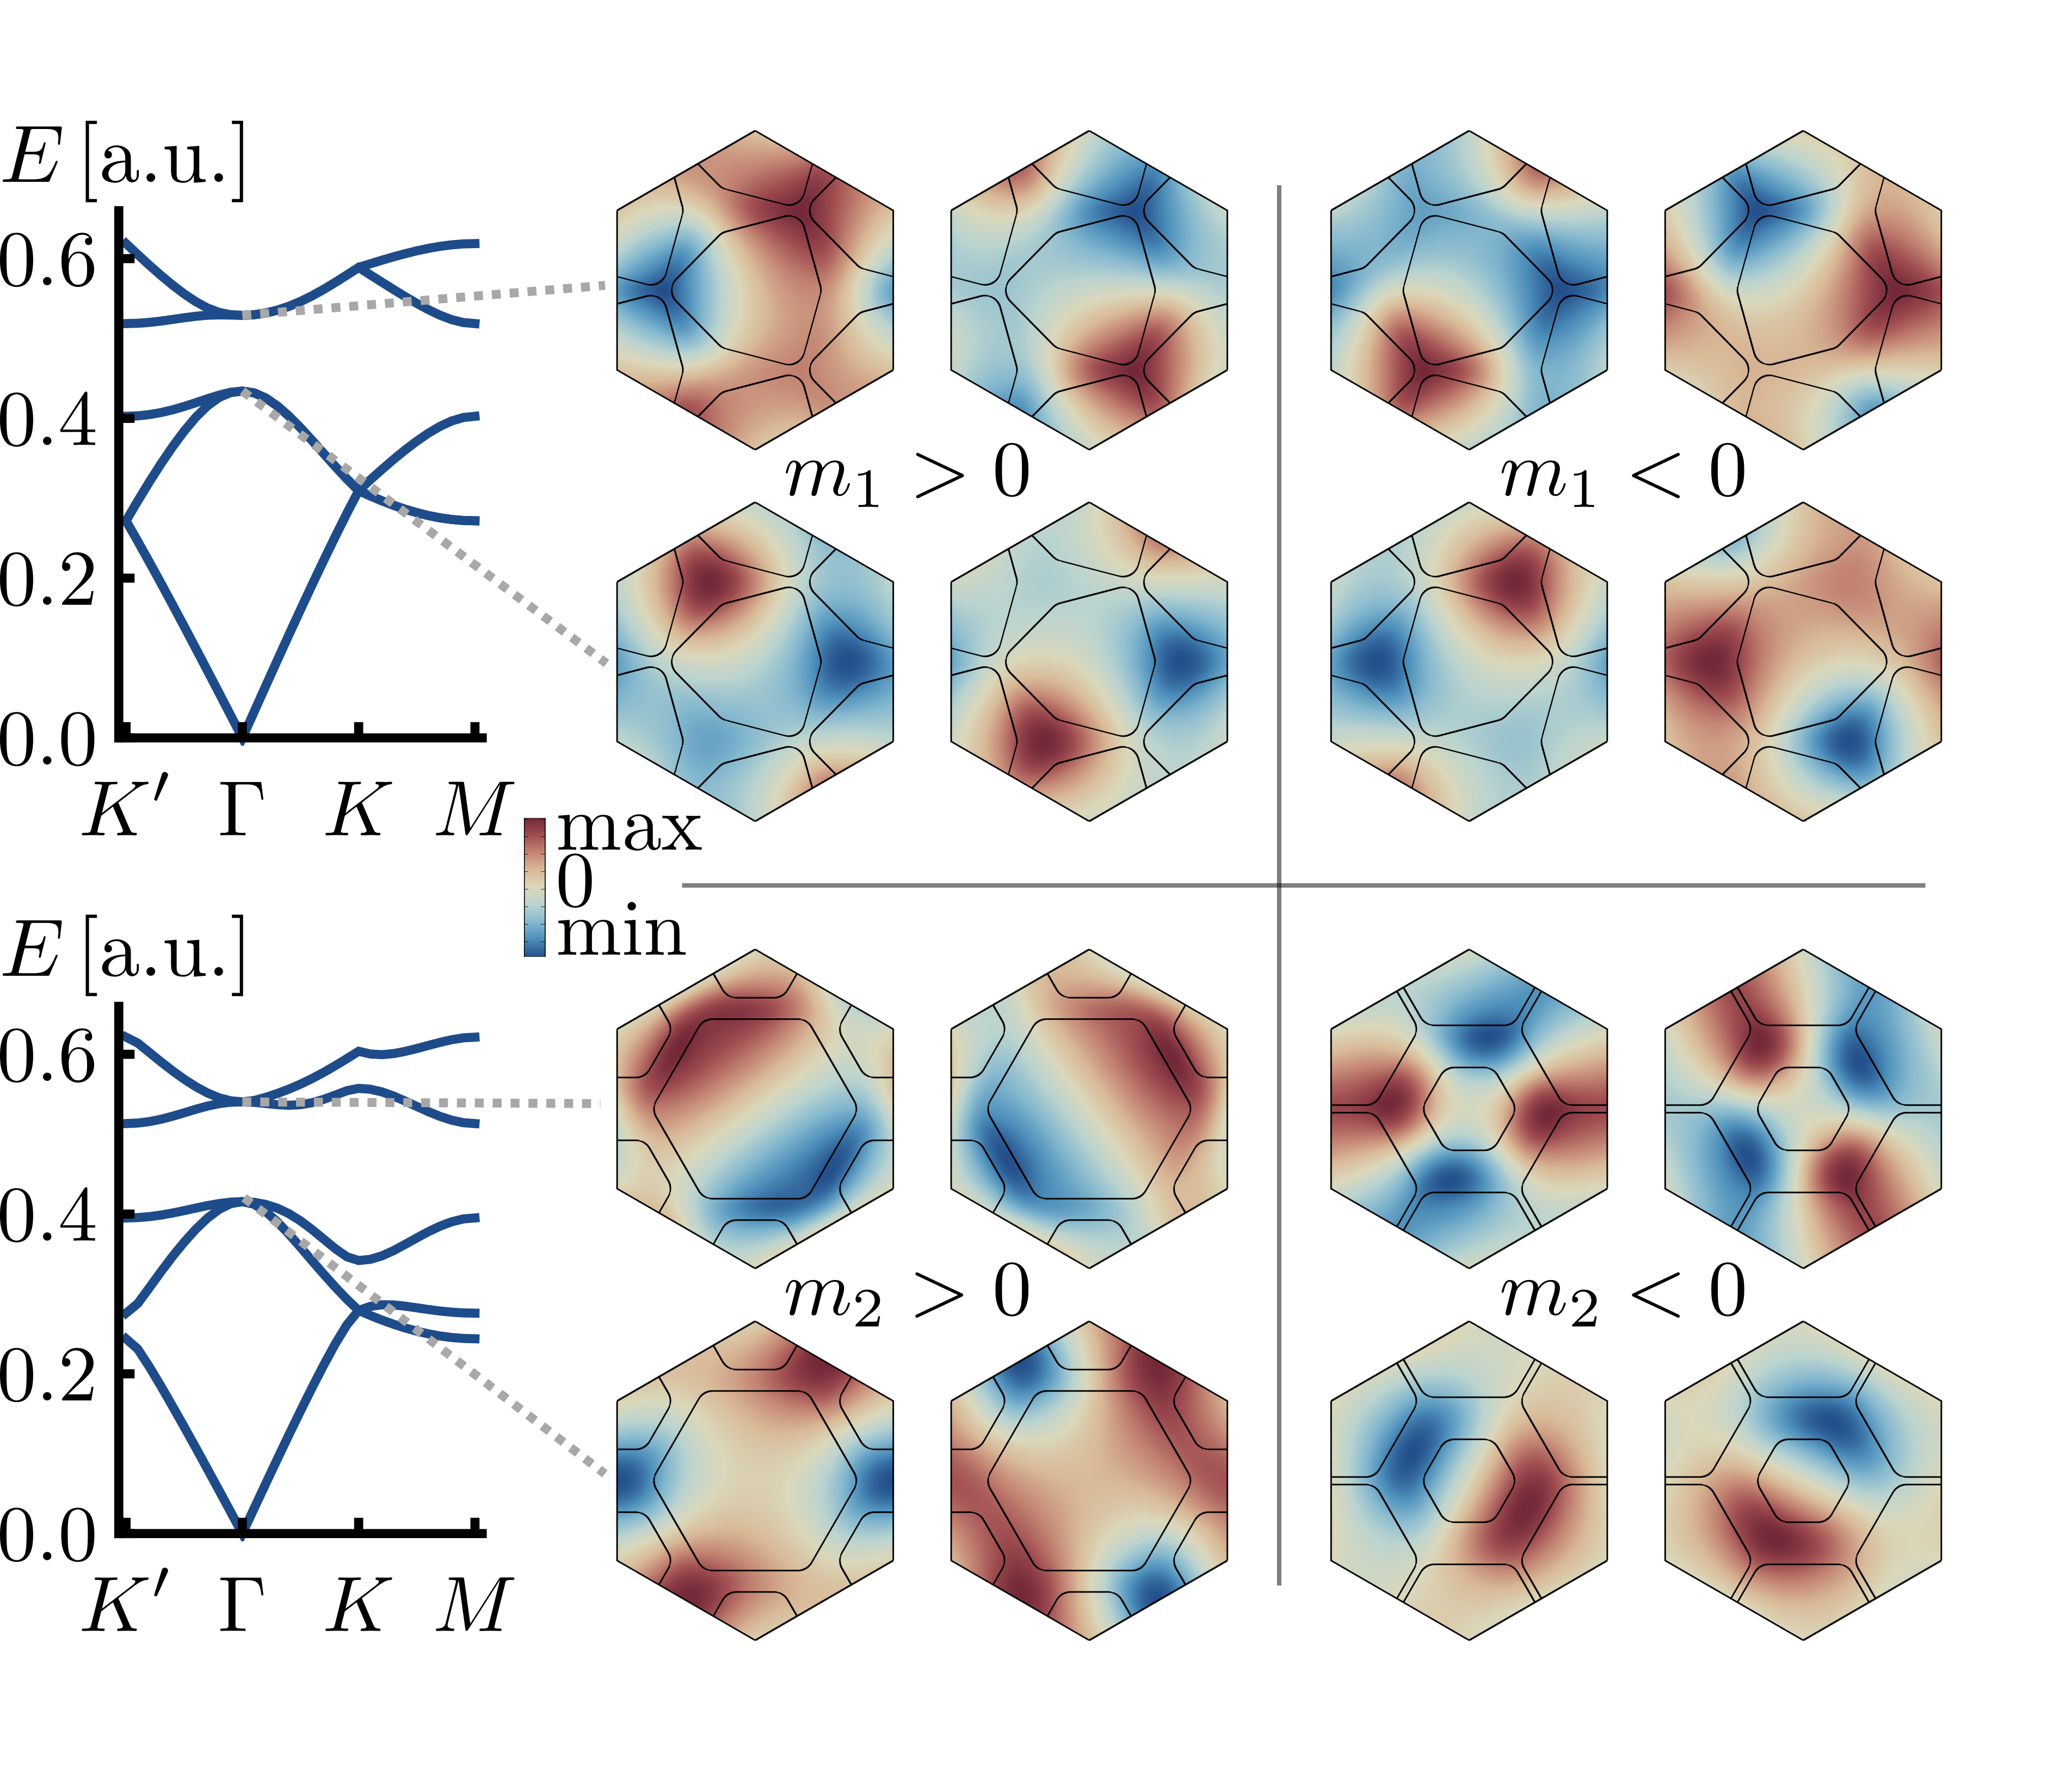
\includegraphics{figures/hoti/fig2.png}
 	\caption{The bulk solutions of the perturbed simple hexagonal lattice using the enlarged unit cell with periodic boundary conditions. The bulk spectrum and the four bulk eigenstates at the $\Gamma$ point below and above the gap for each perturbed unit cell structure, with positive/negative values for each of the symmetry-breaking mass terms. (top) Breaking inversion symmetry [cf.~Table \ref{table:symm_p6m_degs}(b)]. (bottom) Breaking translation symmetry [cf.~Table \ref{table:symm_p6m_degs}(c)].}
 	\label{fig:hoti_bulk_sols}
\end{figure}

\section{Numerical simulations}

\subsection{Bulk signatures of broken symmetry} \label{sec:hoti_bulk}

Our discussion has so far relied on very general symmetry arguments. In Sec.~\ref{sec:symm_sixfold}, we found the matrices corresponding to different perturbations, but no quantitative details, i.e., the "perturbation strengths" $m_1$ and $m_2$ are unknown. We now wish to extract these from bulk simulations of the respective unit cells.

Let us assume we have numerically found a set of eigenstates for our perturbed structure. To extract the mass terms, we again focus on the $\Gamma$ point of the enlarged unit cell and consider the four numerical solutions, $\{ \phi_j(\vb{r})\}$, $j=1,2,3,4$, with eigenvalues $E_j$ and corresponding deviations from mid-gap $\Delta E_j=E_j-\bar{E}$ for $\bar{E}=\sum_j E_j/4$. In the effective $4 \times 4$ model, the mass terms would have been simple to evaluate from the solutions $\{ \vb{v}_j \}$ in the respective basis,
\begin{equation} \label{eq:hoti_proj}
m_i = \Delta E_j \expval{\Gamma_i}{\vb{v}_j} \,,
\end{equation}
with either choice of $j$. 
However, if all we have are the numerical functions $\{ \phi_j (\vb{r}) \}$, we need to perform the projection \eqref{eq:hoti_proj} in real space. To this end, we must convert the matrices $\Gamma_i$ to real-space operations, i.e., invert the mapping $\rho(g)$ introduced in Sec.~\ref{sec:symm_groups}. Averaging over the four solutions then yields
\begin{equation}
\label{eq:hoti_massformula}
m_i = \frac{1}{4} \sum_j \Delta E_j  \int_{\text{cell}} \phi_j^*(\vb{r}) \rho^{-1}(\Gamma_i) \phi_j(\vb{r})  \, dS\,.
\end{equation}
Using the known representation matrices of the various symmetry operations found in Eq.~\eqref{sec:symm_sixfold}, we get
\begin{equation} \label{eq:hoti_bulksig}
\begin{aligned}
\rho^{-1}(\Gamma_1) &= -\left(4C_3 \vb{a} + 2 C_3 + 2 \vb{a} + 1 \right) /\, 3\,, \\
\rho^{-1}(\Gamma_2) &= -C_6^3\,.
\end{aligned}
\end{equation}
If the perturbative approach is sound, the two mass terms should account for the entire bandgap, meaning $\abs{\Delta E_j} = \sqrt{m_1^2 + m_2^2}$ for all $j$.
%Furthermore, if the 2D irreps of the respective subgroups are truly degenerate, the obtained $m_1$ and $m_2$ do not depend on the choice of $\ket{\psi_i}$.

To apply Eq.~\eqref{eq:hoti_massformula} and find the bulk signatures, we must now choose a specific system. We opt for the electromagnetic domain, governed by the wave equation \eqref{eq:symm_maxwell}. To match contemporary experimental work, we select silicon nitride as the bulk material ($\epsilon_r = 11.7$), with vacuum in the incisions ($\epsilon_r = 1$).
%
\begin{figure} [h!]
	\centering
	\hspace*{-5mm}
	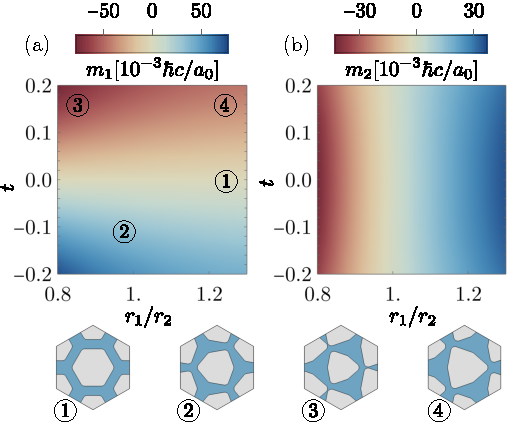
\includegraphics[scale=0.9]{figures/hoti/fig3.pdf}
	\caption{The bulk solutions of the perturbed simple hexagonal lattice using the enlarged unit cell and combining the two kinds of symmetry-breaking deformations, cf.~Fig.~\ref{fig:hoti_bulk_sols}. The (a) $m_1$ and (b) $m_2$ mass terms, extracted using~Eq.~\eqref{eq:hoti_massformula}. The bottom panel shows the unit cell at selected points in the configuration space.}
	\label{fig:hoti_bulk_sig}
\end{figure} 
%
In Fig.~\ref{fig:hoti_bulk_sig}, we plot the dependence of the effective masses $m_1$, $m_2$ on the structural features of the simple hexagonal lattice example, which we saw in Fig.~\ref{fig:hoti_bulk_sols}. Inversion symmetry is broken by deforming the hexagonal incision into a triangle, parameterized by $t$. Translation symmetry is broken by introducing two different radii $r_1$ and $r_2$ for the central and outer hexagonal incisions, parameterized by $r_1/r_2$. Using such a construction, the deformations can be combined in a single unit cell, as shown in Fig.~\ref{fig:hoti_bulk_sig}(1)-(4). The calculations were performed using the COMSOL finite element software~\cite{comsol}. In Fig.~\ref{fig:hoti_bulk_sig}(a),~(b), the mass terms are seen to vary independently under the different symmetry-breaking deformations. This confirms that we can readily realize a spatially-dependent mass term $\boldsymbol{m}(\vb{r})$, as required by the Jackiw-Rossi model. We reiterate that to create a bound mode, the structures used for the winding must have coincident bandgaps.

\subsection{A topological vortex}

We move now to construct a Jackiw-Rossi vortex in a large supercell composed of the different bulk phases. To obtain a topological bound mode, the mass vector must wind [cf.~Eq.~\eqref{eq:invariant}], i.e., we need to spatially pass through all four "pure" perturbations shown in Fig.~\ref{fig:hoti_bulk_sols}. 
Constructing a vortex of $n=1$ in a dielectric medium, we numerically confirm the existence of a bound mode in Fig.~\ref{fig:hoti_fig4}. To ensure an overall bandgap, we use only the four unit cells shown in Fig.~\ref{fig:hoti_bulk_sig}.
%
\begin{figure} [h!]
	\centering
	\includesvg{figures/hoti/fig4_enlarged.svg}
	\caption{Numerical simulation of a Jackiw-Rossi vortex with $n = 1$ in a continuous dielectric ($\epsilon_r = 11.7$) patterned with air incisions. The simulated supercell combines four bulks corresponding to the four perturbed structures in Fig.~\ref{fig:hoti_bulk_sols}. This gives rise to a Jackiw-Rossi vortex~\eqref{eq:hoti_H} at the cell's center. Periodic boundary conditions are used at all four edges of the cell, giving a total of four vortices. (a) The energy spectrum of the structure showing bulk modes (blue fill), edge modes (red fill) and 0D bound modes (white fill). (b) The supercell, showing the signs of the mass terms $(m_1, m_2)$ and boundaries between the phases. The amplitude of a mid-gap solution is overlayed onto the structure, exhibiting a mode bound at the center. Similar plots follow for (c) one of the gapped edge mode solutions and (d) the other vortex sites.}
	\label{fig:hoti_fig4}
\end{figure}
%
Since we use periodic boundary conditions, the supercell features four distinct vortex sites, all with the same $\abs{n}$ but with different terminations\footnote{If a fixed boundary condition is used instead, many new modes appear at the boundary which do not respect the bulk bandgap. Their effect on the central vortex mode is negligible, as its hybridisation with the boundary solutions is minimised by the lack of spatial overlap.}. Correspondingly, we find four bound modes, each localized at one of the four vortices. By construction, the topological vortex modes should appear mid-gap. One of the vortex modes indeed lies at the bulk gap center, while the remaining three deviate slightly away [see Fig.~\ref{fig:hoti_fig4}(a)]. We attribute this discrepancy to the inequivalent vortex terminations, where the spatial symmetries are locally broken~\cite{Gao_2020}. Note that gapped topological edge states exist at the domain walls between different mass regions, as expected in second-order topological insulators~\cite{Benalcazar_2017a,Benalcazar_2017b,Petrides_2020}, see Figs.~\ref{fig:hoti_fig4}(a)~and~(c). These gapped edge states can be interpreted gapped 1D bulks, which undergo a band inversion at the position of the central vortex, creating a boundary mode there.  

\section{Discussion}

We highlight that our analysis is applicable to a broad range of geometries and systems, as it relies solely on the symmetries of the perturbations and on time reversal. Moreover, our construction does not rely on introducing pseudo-spin or pseudo-time reversal symmetries~\cite{Wu_Hu_2015}. Instead, the initial 4-fold degeneracy is directly obtained by starting with the original unit cell and its associated space group. As a side note, we can directly verify that our construction falls into the BDI class of topological insulators~\cite{Teo_2010}, which is defined by possessing time-reversal and chiral symmetries, $\rho(\mathcal{T}) ,\, \rho(\mathcal{C})$, such that $\rho(\mathcal{T})^2 = \rho(\mathcal{C})^2 = 1$. In our chosen 4D basis, time reversal is represented by $\rho(\mathcal{T}) = \left( \tau_1 \otimes \mathbb{1}_2 \right) \mathcal{K}$, where $\mathcal{K}$ is the complex conjugation operator, see Eq.~\eqref{eq:symm_six_rhos}. Chiral symmetry must anticommute with the Hamiltonian -- this is also present, with $\rho(\mathcal{C}) = \tau_2 \otimes \mathbb{1}_2$. The Hamiltonian obeys these due to the spatial symmetries required by our construction. Since $\rho(\mathcal{C})^2 = \rho(\mathcal{T})^2 = 1$, our system belongs to the BDI class~\cite{Chiu_2016, Teo_2010} and thus admits a topological winding number [cf.~Eq.~\eqref{eq:invariant}].

Compared with standard 0D modes formed at non-topological lattice defects (see Sec.~\ref{sec:intro_spatial}), topological vortex modes offer several advantages~\cite{Gao_2020}. (i) Their frequency is near mid-gap, resulting in better spatial confinement and quality factors. (ii) The number of modes formed is fixed by topology.  (iii) The modal area is scalable, as the modes form independently of the vortex size. These aspects make topological vortex modes promising candidates for the construction of single-mode semiconductor lasers. From a technological standpoint, the bulk bandgap size is the key characteristic to keeping the vortex modes spectrally isolated and spatially confined. In Fig.~\ref{fig:hoti_fig4}(a), its size relative to the gap center is $16.6\%$, which is a factor of $3$ higher compared to existing works based on the graphene-inspired TB model~\cite{Gao_2020}. Further improvement is expected with the use of numerical optimization enabled by our work. We also highlight that our scheme can be extended to three dimensions by appropriately extruding the geometry in the out-of-plane direction. This yields one-dimensional, counter-propagating topological modes that can be used to construct optical fibers~\cite{Lin_2020, Lu_2018}.

Finally, we emphasize that the symmetry arguments describe the behaviour of the bands near the high-symmetry points of the BZ, but do not guarantee a fully gapped spectrum. In the Kagome lattice, for example, a dielectric patterned with air incisions shows the correct symmetry breaking at the $\Gamma$ point, but the spectrum is gapless due to the band dispersion at other regions of the BZ, yielding only an indirect gap at the $\Gamma$ point. Such limitations are peculiar to specific experimental platforms. 

